\documentclass[russian,utf8,emptystyle]{eskdtext}

\usepackage[T2A,T1]{fontenc}

\newcommand{\No}{\textnumero} % костыль для фикса ошибки

\ESKDdepartment{Федеральное государственное бюджетное образовательное учреждение высшего профессионального образования}
\ESKDcompany{Московский государственный технический университет им. Н. Э. Баумана}
\ESKDclassCode{23 0102}
\ESKDtitle{АИС отслеживания и прогнозирования новостных потоков «Волхв»}
\ESKDdocName{Расчетно-пояснительная записка}
\ESKDauthor{Гуща~А.~В.}
\ESKDtitleApprovedBy{~}{~\underline{\hspace{2.5cm}}}
\ESKDtitleAgreedBy{~}{~\underline{\hspace{2.5cm}}}
\ESKDtitleDesignedBy{Студент группы ИУ5-122}{Гуща~А.~В}

\usepackage{multirow}
\usepackage{tabularx}
\usepackage{tabularx,ragged2e}
\usepackage{pdfpages}
\renewcommand\tabularxcolumn[1]{>{\Centering}p{#1}}
\newcommand\abs[1]{\left|#1\right|}

\usepackage{longtable,tabu}

\usepackage{geometry}
\geometry{footskip = 1cm}

\pagenumbering{arabic}
\pagestyle{plain}

\usepackage{setspace}

\usepackage{xcolor}
\usepackage{listings}
\lstset{
    breaklines=true,
    postbreak=\raisebox{0ex}[0ex][0ex]{\ensuremath{\color{red}\hookrightarrow\space}},
    extendedchars=\true,
    basicstyle=\small,
    inputencoding=utf8,
    numbers=left,                    
    numbersep=5pt,                  
    numberstyle=\tiny\color{mygray},
}
\renewcommand{\lstlistingname}{Листинг}
\renewcommand{\lstlistlistingname}{Листинги}

\ESKDsectAlign{section}{Center} % to capitalize russian text

\usepackage{array}
\newcolumntype{L}[1]{>{\raggedright\let\newline\\\arraybackslash\hspace{0pt}}m{#1}}
\newcolumntype{C}[1]{>{\centering\let\newline\\\arraybackslash\hspace{0pt}}m{#1}}
\newcolumntype{R}[1]{>{\raggedleft\let\newline\\\arraybackslash\hspace{0pt}}m{#1}}

\usepackage{tikz}
\usepackage{pgf-pie}

\usepackage{totcount}
\regtotcounter{figure}
\regtotcounter{table}

%\usepackage{titlesec}
\usepackage{hyperref}

\setcounter{secnumdepth}{5}
\setcounter{tocdepth}{5}

%\renewcommand*{\thesection}{\arabic{section}}

%===========================================================================
\begin{document}

\clearpage
\clearpage

\section*{Реферат}
%\pageref{LastPage}
Данная расчетно-пояснительная записка содержит 154 (без приложения) страниц, \total{figure} иллюстраций (без приложения), \total{table} таблиц, 1 приложение, 24 использованных источников.

Ключевые слова: полнотекстовый поиск, сбор информации, формальный язык запросов, генетическое программирование, эволюционные алгоритмы, символьная регрессия, прогноз временных рядов.

Данный дипломный проект посвящен разработке автоматизированной информационной системы для анализа новостных потоков, а также прогнозирования их активности. Целью разработки является сбор информации из открытых источников, накопление данной информации в СУБД, проведение анализа накопленных новостных данных на основе проблемно ориентированного языка программирования и предсказание количества новостей по определенной тематике с помощью эволюционных методов прогнозирования.

Система проектируется в виде веб-сервиса, предоставляющих пользователю набор экранных форм для взаимодействия с данным программных изделием, а также машинный интерфейс для взаимодействия стороннего программного обеспечения с данной АИС. Структуру системы составляют сервер приложения, сервер СУБД, сервер индексации и терминалы пользователей. При разработке программного продукта используется язык программирования Haskell.

В результате разработки была спроектирована автоматизированная информационная система, отвечающая требованиям технического задания и имеющая возможности, необходимые как для сбора и хранения новостной информации в базах данных, так и для всестороннего ее анализа.

Область применения АИС -- лаборатории анализа данных, составной компонент в распределённых системах анализа данных. Проект является некоммерческим с малой стоимостью выполнения.

\tableofcontents

\section*{Нормативные ссылки}

В дипломном проектировании использованы следующие стандарты:
\begin{itemize}
\item ГОСТ 2.105-95 -- «ЕСКД. Общие требования к текстовым документам».
\item ГОСТ 7.1-2003  -- «СИБИД. Библиографическая запись. Библиографическое описание. Общие требования и правила составления».
\item ГОСТ 7.12-93 -- «СИБИД. Библиографическая запись. Сокращение слов на русском языке».
\item ГОСТ 7.32-2001 -- «СИБИД. Отчет о научно-исследовательской работе. Структура и правила оформления».
\item ГОСТ 19.701-90 -- «ЕСКД. Схемы алгоритмов, программ, данных и систем. Условные обозначения и правила выполнения».
\item СанПиН 2.2.1/2.1.1.1278-03 -- «Гигиенические требования к естественному, искусственному и совмещенному освещению жилых и общественных зданий».
\item СанПиН 2.2.2/2.4.1340-03 -- «Гигиенические требования к видеодисплейным терминалам, персональным электронно-вычислительным машинам и организации работы».
\item СНиП 2.04.05-86  --  «Отопление, вентиляция и кондиционирование».
\end{itemize}

В расчетно-пояснительной записке имеются ссылки на следующие стандарты:
\begin{itemize}
\item ГОСТ 12.1.002-84 -- «ССБТ. Электрические поля промышленной частоты. Допустимые уровни напряженности и требования к проведению контроля на рабочих местах».
\item ГОСТ 12.1.003-83 -- «ССБТ. Шум. Общие требования безопасности».
\item ГОСТ 12.1.004-91 -- «ССБТ. Пожарная безопасность. Общие требования».
\item ГОСТ 12.1.005-88 -- «ССБТ. Общие санитарно-гигиенические требования к воздуху рабочей зоны».
\item ГОСТ 12.1.006-84 -- «ССБТ. Электромагнитные поля радиочастот. Допустимые уровни на рабочих местах и требования к проведению контроля».
\item ГОСТ 12.2.007.3-75 -- «ССБТ. Электротехнические устройства на напряжение свыше 1000 В. Требования безопасности».
\item ГОСТ 12.2.007.4-75 -- «ССБТ. Шкафы комплектных распределительных устройств и комплектных трансформаторных подстанций, камеры сборные одностороннего обслуживания, ячейки герметизированных элегазовых распределительных устройств».
\item ГОСТ 12.1.010-76 -- «ССБТ. Взрывобезопасность. Общие требования».
\item ГОСТ 12.1.018-93 -- «ССБТ. Пожаровзрывобезопасность статического электричества. Общие требования».
\item ГОСТ 12.1.038-82 -- «ССБТ. Электробезопасность. Предельно допустимые значения напряжений прикосновения и токов».
\item ГОСТ 12.1.045-84 -- «ССБТ. Электростатические поля. Допустимые уровни на рабочих местах и требования к проведению контроля».
\item ГОСТ 12.4.124-83 -- «ССБТ. Средства защиты от статического электричества. Общие технические требования».
\item СанПиН 2.2.4.548-96 -- «Гигиенические требования к микроклимату производственных помещений».
\item СНиП 23-05-95 -- «Естественное и искусственное освещение».
\end{itemize}
\section*{Определения, обозначения и сокращения}

\begin{itemize}
\item АПК -- аппаратно-программный комплекс.
\item БД -- база данных.
\item ЕСКД -- единая система конструкторской документации.
\item Управляющий класс (control) -- класс модели анализа, представляющий координацию, последовательность и управление другими объектами, часто используется для инкапсуляции управления для варианта использования.
\item Граничный класс (boundary) -- класс модели анализа, используемый для моделирования взаимодействия между системой и ее актантами, то есть пользователями и внешними системами.
\item Класс сущности (entity) -- класс модели анализа, используемый для моделирования долгоживущей, часто персистентной информации.
\item ОЗУ -- оперативное запоминающее устройство.
\item ОС -- операционная система.
\item ПК -- персональный компьютер.
\item ПО -- программное обеспечение.
\item ПЭВМ -- персональная электронно-вычислительная машина.
\item СанПиН -- санитарно-эпидемиологические правила и нормативы.
\item СИБИД -- система стандартов по информации, библиотечному и издательскому делу.
\item СНиП -- строительные нормы и правила. 
\item ССБТ -- система стандартов по информации, библиотечному и издательскому делу.
\item СУБД -- система управления базами данных.
\item ЭВМ -- электронно-вычислительная машина.
\item ЭМП -- электромагнитное поле.
\item API -- application programming interface -- набор готовых классов, процедур, функций, структур и констант, предоставляемых приложением (библиотекой, сервисом) для использования во внешних программных продуктах.
\item CPU -- central processing unit -- центральный процессор.
\item HDD -- hard disk drive -- жесткий диск.
\item SQL -- structured query language -- универсальный компьютерный язык, применяемый для создания, модификации и управления данными в реляционных базах данных. SQL основывается на исчислении кортежей. SQL является, прежде всего, информационно-логическим языком, предназначенным для описания, изменения и извлечения данных, хранимых в реляционных базах данных. 
\item UML -- unified modeling language, унифицированный язык моделирования -- язык графического описания для объектного моделирования в области разработки программного обеспечения. UML является языком широкого профиля, это открытый стандарт, использующий графические обозначения для создания абстрактной модели системы, называемой UML-моделью.
\end{itemize}
\section*{Введение}

Дипломный проект на тему <<Автоматизированная информационная система отслеживания и прогнозирования новостных потоков <<Волхв>> >> посвящен созданию системы, которая позволит накапливать информацию из открытых источников СМИ, аналитических материалов экспертов, социальных сетей, а также предоставит инструменты для всестороннего анализа накопленной информации. АИС <<Волхв>> предоставляет два способа анализа накопленной новостной информации: с помощью проблемно-ориентированного языка запросов и с помощью автоматизированного прогнозирования количества сообщений, удовлетворяющих заданному запросу.



%===========================================================================
% Конструкторская часть
\section{Конструкторская часть}

\subsection{Постановка задачи проектирования}

Автоматизированная информационная система отслеживания и прогнозирования новостных потоков «Волхв» позволяет проводить накопление и анализ новостных документов с помощью формализованного языка запросов для полнотекстового поиска информации. Данная АИС предназначена для исследовательской деятельности и для включения в состав сложных комплексов анализа событий в новостных потоках.

АИС «Волхв» должна выполнять следующие функции:
\begin{itemize}
\item Удаленный доступ к системе. Программное изделие должно обеспечивать удаленный доступ на получение информации к системе через Web-сервер.
\item Соединение с базой данных. Программное изделие должно осуществлять удаленное соединение с базой данных.
\item Ввод с клавиатуры. Данные, вводимые с клавиатуры должны иметь тип и формат, соответствующий типу и формату полей записи.
\item Добавление информации в базу данных. Программное изделие должно осуществлять добавление новой записи в базу данных при условии, что эта запись удовлетворяет всем требованиям, налагаемым на входные данные.
\item Удаление информации из базы данных. Программное изделие должно осуществлять исключение выбранной пользователем записи в таблице из исходной базы данных.
\item Редактирование информации в базе данных. Функция должна осуществлять редактирование поля записи, выбранного пользователем. При этом при редактировании данных должны выполняться все требования, налагаемые на входные данные.
\item Выполнение поисковых запросов. Программное изделие должно выполнять поисковые запросы на проблемно-ориентированном языке и отображать результаты их выполнения пользователю.
\item Выполнение прогнозирования новостных потоков. Программное изделие должно производить краткосрочные прогнозы количества документов, соответствующих заданному запросу.
\item Предоставление машинного интерфейса интеграции. Программное изделие должно предоставлять машинный Web-интерфейс, который позволит интегрировать данную АИС в составные комплексы.
\end{itemize}


\clearpage
\subsection{Описание предметной области}
\subsubsection{Естественно-языковая модель предметной области}

На данный момент существует очень мало систем, позволяющих проводить полнотекстовый поиск по документам на основе формализованного языка запросов, которые можно включить в состав автономной системы.

АИС «Волхв» должна агрегировать новостные документы из разных новостных источников, которые поступают в систему либо через пользователя, либо от автоматических роботов сбора. Все новые документы проходят индексацию для возможности быстрого полнотекстового поиска по тексту документа. Полнотекстовый поиск должен учитывать морфологию языка (система поддерживает русский и английский язык), то есть «отмечаемому» и «отмечать» должны быть найдены при полнотекстовом поиске «отмечает».

Аналитик или исследователь может использовать АИС «Волхв» для исследований в области «big data» или включить данную АИС в состав программного комплекса для проведения сложного составного анализа новостных событий с помощью формализованного языка запросов. 

Формализованные запросы могут быть использованы для таких задач как:
\begin{itemize}
\item Выявление событий в тексте. Специально составленный формализованный запрос определяет наличие события, его тему и дату. После этого необходима дополнительная обработка результатов запроса для проведения кластеризации событий и определения связей между ними.
\item Геотегирование текстов. Формализованный запрос может определять географические привязки новостных сообщений путем учета упоминаемых географических названий. К результатам такого запроса можно привязать географические метки, чтобы использовать их в более сложных запросах.
\item Определение эмоциональной окрашенности текстов. Формализованный запрос определяет слова-маркеры с эмоциональной окраской, считает суммарную оценку эмоциональной окраски и отмечает текст специально меткой, которую можно использовать в остальных запросах.
\item Отслеживание потоков распространения информации. Аналитик подготавливает формализованных запрос, который реагирует на конкретное сообщение о недавнем событии. Используя сравнение дат и источников результатов запроса, аналитик может определить первоисточники информации и источники, которые являются вторичными. 
\item Извлечение знаний из текстов. Среди новостных текстов об событиях присутствуют аналитические тексты, из которых возможно извлечение фактов и логических связей между ними. С помощью формализованных запросов можно обнаруживать такие тексты и извлекать предложения, которые содержат знания. Результаты таких формализованных запросов нуждаются в последующей обработке для преобразования знаний в необходимый формат.
\end{itemize}

Для реализации перечисленных задач предлагается использовать системы полнотекстового поиска. Такие системы позволяют строить индекс по тексту документа. Данный индекс позволяет ускорить поиск по тексту документа и учитывать при поиске морфологические особенности языки. Для поискового запроса <<кошка>> система должна найти документы с различными формами этого слова: кошек, кошки, кошку. Но простого поиска с учетом морфологии недостаточно для проведения аналитики, необходимо вычислять и учитывать сложные параметра текста, например:
\begin{itemize}
\item Расстояния между словами. В реальных текстах интересующие аналитика слова зачастую разделены несколькими дополнительными словами. Данная метрика помогает наложить ограничение на максимальное расстояние между словами в поисковом запросе.
\item Расположение относительно начала и конца текста. Данное ограничение позволяет искать документы с заданными введениями и заключениями.
\item Расположение относительно начала и конца предложений. С помощью данной метрики можно наложить ограничение на присутствие поисковых слов в пределах одного предложения.
\item Составные метрики с помощью логических операций. Объединение метрик и поисковых слов в составные запросы с помощью И, ИЛИ или логического отрицания необходимы для создания запросов, полезных на практике. 
\end{itemize}

При выполнении формализованного запроса также необходимо иметь возможность накладывать ограничения на даты публикации текстов, источники документов, наличие специальных меток от предыдущих запросов. Совокупность метрик и ограничений на результаты поиска формируют проблемно ориентированный язык для описания таких формализованных запросов. Ниже приведён формализованный запрос для определения документов о коррупции в Карелии за период от Января 2016 до Апреля 2016.

\begin{verbatim}
SELECT id, weight() FROM rt WHERE MATCH('
  ( взятка 
  | (злоупотребление NEAR/5 должностными NEAR/5 полномочиями) 
  | (злоупотребление NEAR/5 служебным NEAR/5 положением) 
  | (дача NEAR/5 взятки) 
  | (получение NEAR/5 взятки)) 
  (Карелия | Петрозаводск) ') 
  AND timestamp > 1451606400 
  AND timestamp < 1461283200 
  ORDER BY weight() DESC LIMIT 0,50 OPTION max_matches=10000000 
\end{verbatim}

В результате выполнения формализованных запросов аналитик получает выборку документов, которые подходят под условия этого запроса. Для анализа результатов зачастую необходимо знать, как ведут себя результаты запроса во времени и как они будут себя вести в будущем. Поэтому в АИС реализовано отображение графиков формализованных запросов по дням и краткосрочное прогнозирование. Прогнозирование производится всё время работы системы с постепенным уточнением. Используется метод символьной регрессии на основе эволюционных алгоритмов, описанных в части 3 данного документа. В результате прогнозирования аналитик получает не только график прогноза, но и аналитическую формулу этого графика.

Предметная область разработанной автоматизированной системы представлена на
рисунке~\ref{figure:domain}.

\begin{figure}[!h]
\centering
\includegraphics{design/domain}
\caption{Схема предметной области АИС.}
\label{figure:domain}
\end{figure}

\subsubsection{Сущности предметной области}

В процессе предварительного анализа предметной области были выделены следующие основные сущности:
\begin{itemize}
\item Документ;
\item Рубика;
\item Запрос;
\item Прогноз;
\item Формула;
\end{itemize}

А также дополнительные сущности, наличие которых следует из предыдущих:
\begin{itemize}
\item Метка документа;
\item Приложение документа;
\item Источник документа;
\item Операция системы -- долгосрочные операции над базой документов;
\item Настройки системы -- настройки пользователя.
\item Измерение прогноза -- сохранённый результат выполнения запроса прогноза по дням;
\item Популяция прогноза -- коллекция формул для прогноза;
\item Приспособленность -- история лучших и средних значений функции приспособленности по поколениям для популяции;
\end{itemize}

\subsubsection{Перечень процессов, подлежащих автоматизации}
Автоматизации подлежат следующие процессы системы:
\begin{itemize}
\item Ввод документа в систему;
\item Построение ускоряющего поиск индекса;
\item Выполнение полнотекстового поиска на основе формализованного языка
запросов;
\item Просмотр документов и их редактирование;
\item Выполнение операций над индексом;
\item Рубрикация документов и сохранённых запросов;
\item Прогнозирование новостных потоков.
\end{itemize}

\subsubsection{Выбор и обоснование критериев качества}

Для данного программного изделия можно выделить следующие критерии качества:
\begin{itemize}
\item Удобство пользовательского интерфейса;
\item Качество полнотекстового поиска;
\item Дизайн рубрикатора;
\item Удобство интеграции с другими системами;
\item Возможность отмечать документы метками;
\item Качество прогноза.
\end{itemize}

\paragaph{Удобство пользовательского интерфейса.}
Означает простоту и понятность работы с системой. Оценивается:
\begin{itemize}
\item структура сайта (доступ к любой странице сайта требует не более трех кликов);
\item наличие сквозного меню (меню, которое присутствует на каждой странице сайта);
\item присутствие на всех страницах сайта ссылки на главную страницу;
\item иерархическая структурированность информации сайта, степень интуитивно понятного меню;
\end{itemize}

\paragraph{Качество полнотекстового поиска.}
Оценка релевантности найденной информации, скорость выполнения запроса, возможности формализованного языка запросов.

\paragraph{Дизайн рубрикатора.}
При оценке дизайна рубрикатора документов учитывается:
\begin{itemize}
\item Непосредственное наличие рубрикатора в стандартной поставке системы;
\item Стиль отображения древовидной структуры;
\item Отображение сохранённых запросов внутри рубрик;
\item Отображение информации о количестве документов в рубрике;
\end{itemize}

\paragraph{Удобство интеграции с другими системами.} 
Оценивается:
\begin{itemize}
\item Наличие интеграционного интерфейса;
\item Удобность этого интерфейса для разработчиков;
\item Полнота интерфейса (полная реализация всех возможностей системы в интерфейсе).
\end{itemize}

\paragraph{Возможность отмечать документы метками.}
Наличие возможности отмечать произвольными метками документы или сложность реализации такой возможности. Включает в себя:
\begin{itemize}
\item Поиск по наличию меток или по их отсутствию;
\item Удобство отображения для пользователя;
\item Возможность пользователю задавать метки документам;
\item Удобство интеграционного интерфейса для работы с метками.
\end{itemize}

\paragraph{Качество прогноза.}
При оценке качества прогноза новостного потока учитывается:
\begin{itemize}
\item Построение графиков количества документов, соответствующих сохранённому запросу, по дням;
\item Наличие ретроспективного прогноза;
\item Отображение аналитической функции прогноза;
\item Качество прогнозирования, возможность прогнозировать сложные потоки;
\end{itemize}

Присвоим критериям качества следующие весовые коэффициент, которые отображены в таблице~\ref{table:qualityWeights}.

\begin{table}[h!]
\centering
\caption{Критерии качества и их весовые коэффициенты}
\label{table:qualityWeights}
\begin{tabular}{L{10cm}|C{3cm}}
\multicolumn{1}{C{10cm}|}{Критерий} & 
\multicolumn{1}{C{3cm}}{$\alpha$} \\
\hline\hline

Удобство пользовательского интерфейса & 0.1 \\
Качество полнотекстового поиска & 0.4 \\
Дизайн рубрикатора & 0.1 \\
Удобство интеграции & 0.2 \\
Возможность отмечать документы метками & 0.1 \\
Качество прогноза & 0.1 \\

\end{tabular}
\end{table}

Выполнено следующее условие:
\begin{equation}
\sum \alpha_i = 0.1 + 0.4 + 0.1 + 0.2 + 0.1 + 0.1 = 1
\end{equation}

\subsubsection{Перечень задач, подлежащих решению в процессе разработки}

В процессе разработки необходимо решить следующие задачи:
\begin{itemize}
\item исследование и анализ предметной области;
\item анализ и определение критериев качества;
\item определение функциональных требований для разрабатываемой системы;
\item разработка структуры модулей системы, с выделением функциональности для каждого модуля;
\item проектирование базы данных: инфологической и даталогической модели;
\item проектирование эволюционного алгоритма прогнозирования, исследование его сходимости;
\item рассмотрение и обоснование архитектурных особенностей реализации системы;
\item выбор программных библиотек для реализации модулей;
\item разработка интерфейса взаимодействия пользователя с программой;
\item написание и отладка программного кода модулей системы;
\item разработка технической документации.
\end{itemize}

\subsubsection{Анализ аналогов и прототипов}

Для расчета нормированного значения j-го варианта по i-ому критерию необходимо
воспользоваться формулой~\ref{equation:criteria}.

\begin{equation}
\label{equation:criteria}
K_{ij} = \frac{x_{ij} - x_i^-}{x_i^+ - x_i^-}
\end{equation}
\begin{ESKDexplanation}
\item[где ] $x_{ij}$ - натуральное значение;
\item       $x_i^+$ - максимальное значение;
\item       $x_i^-$ - минимальное значение.
\end{ESKDexplanation}

Для расчета интегрального показателя необходимо воспользоваться формулой~\ref{equation:criteriaTotal}.

\begin{equation}
\label{equation:criteriaTotal}
K = \sum_{i=1}^m \alpha_i K_{ij}
\end{equation}
\begin{ESKDexplanation}
\item[где ] $m$ - количество критериев.
\end{ESKDexplanation}

Оценка по критериям производится путём присуждения баллов в соответствии со шкалой, представленной в таблице~\ref{table:criteria}.

\begin{table}[h!]
\centering
\caption{Критерии качества и их весовые коэффициенты}
\label{table:criteria}
\begin{tabular}{L{4cm}|C{2cm}|C{2cm}|C{2cm}|C{2cm}|C{2cm}}
\multicolumn{1}{C{4cm}|}{Качественный показатель} & 
\multicolumn{1}{C{2cm}|}{Отлично} & 
\multicolumn{1}{C{2cm}|}{Хорошо} & 
\multicolumn{1}{C{2cm}|}{Удовлетворительно} & 
\multicolumn{1}{C{2cm}|}{Плохо} & 
\multicolumn{1}{C{2cm} }{Неудовлетворительно} \\
\hline\hline

Количественный показатель & 5 & 4 & 3 & 2 & 1 \\
$K_{ij}$ & 1 & 0.75 & 0.5 & 0.25 & 0 \\

\end{tabular}
\end{table}

Исследуем три системы аналогов:
\begin{itemize}
\item Elsatic search
\item Mircrosoft search server
\item ODB Text
\end{itemize}

Эти аналоги имеют ряд принципиальных недостатков и не могут отвечать всем
требованиям.

Недостатками аналога «Elsatic search» являются:
\begin{itemize}
\item отсутствие системы прогнозирования;
\item отсутствие готового интерфейса пользователя.
\end{itemize}

Недостатками аналога «Mircrosoft search server» являются:
\begin{itemize}
\item малое количество возможностей у формализованного языка запросов;
\item отсутствие сохранённых запросов в рубрикаторе;
\item отсутствие системы прогнозирования.
\end{itemize}

Недостатками аналога «ODB Text» являются:
\begin{itemize}
\item невозможность интеграции системы в комплекс;
\item слабая система прогнозирования;
\item отсутствие возможности отмечать документы метками;
\end{itemize}

Сравним аналоги и прототипы без учета весовых коэффициентов, результаты сведены в таблицу~\ref{table:analogs1}.

\begin{table}[h!]
\centering
\caption{Сравнение аналогов и прототипов без учета весовых коэффициентов}
\label{table:analogs1}
\begin{tabular}{L{4cm}|C{3cm}|C{3cm}|C{3cm}|C{3cm}}
\multicolumn{1}{C{4cm}|}{Критерий} & 
\multicolumn{1}{C{3cm}|}{Elastic Search} & 
\multicolumn{1}{C{3cm}|}{Microsoft SC} & 
\multicolumn{1}{C{3cm}|}{ODB Text} & 
\multicolumn{1}{C{3cm}}{Волхв} \\
\hline\hline

Удобство пользовательского интерфейса & 1 & 4 & 5 & 4 \\ \hline
Качество полнотекстового поиска & 5 & 3 & 3 & 5 \\ \hline
Дизайн рубрикатора & 1 & 3 & 4 & 5 \\ \hline
Удобство интеграции & 5 & 3 & 1 & 4 \\ \hline
Возможность отмечать документы метками & 4 & 5 & 1 & 5 \\ \hline
Качество прогноза & 1 & 1 & 3 & 5 \\ \hline
\hline
Итого & 17 & 19 & 17 & 28 \\

\end{tabular}
\end{table}

Сравним аналоги и прототипы с учетом весовых коэффициентов, результаты сведены в таблицу~\ref{table:analogs2}.

\clearpage
\begin{table}[h!]
\centering
\caption{Сравнение аналогов и прототипов c учетом весовых коэффициентов}
\label{table:analogs2}
\begin{tabular}{L{3cm}|C{1cm}|C{3cm}|C{2cm}|C{3cm}|C{3cm}}
\multicolumn{1}{C{3cm}|}{Критерий} & 
\multicolumn{1}{C{1cm}|}{$\alpha$} & 
\multicolumn{1}{C{3cm}|}{Elastic Search} & 
\multicolumn{1}{C{2cm}|}{Microsoft SC} & 
\multicolumn{1}{C{3cm}|}{ODB Text} & 
\multicolumn{1}{C{3cm}}{Волхв} \\
\hline\hline

Удобство пользовательского интерфейса & 0.1 & 0 & 0.75 & 1 & 0.75 \\ \hline
Качество полнотекстового поиска & 0.4 & 1 & 0.5 & 0.5 & 1 \\ \hline
Дизайн рубрикатора & 0.1 & 0 & 0.5 & 0.75 & 1 \\ \hline
Удобство интеграции & 0.2 & 1 & 0.5 & 0 & 0.75 \\ \hline
Возможность отмечать документы метками & 0.1 & 0.75 & 1 & 0 & 1 \\ \hline
Качество прогноза & 0.1 & 0 & 0 & 0.5 & 1 \\ \hline
\hline
Итого & 1 & 0.675 & 0.525 & 0.425 & 0.925 \\

\end{tabular}
\end{table}

Таким образом, автоматизированная информационная система мониторинга и
прогнозирования новостных потоков «Волхв» является лучшим среди аналогов и
оправдывает свое создание.
\subsection{Внутренне проектирование}
\subsubsection{Разработка структуры системы}
\subsubsection{Проектирование структуры базы данных}
\subsubsection{Разработка архитектуры АСОИУ}
\paragraph{Проектирование структуры базы данных} \hfill

Проектирование структуры БД является очень важным этапом, от которого зависят последующие этапы разработки АИС. Время, затраченное разработчиком на проектирование схемы БД, обычно окупается высокой скоростью реализации проекта.

На этапе внешнего проектирования связанного с анализом предметной области были выделены объекты, которые должны использоваться для представления предметной области. То есть была проведена предварительная структуризация объектов предметной области: объекты реального мира подверглись классификации, была зафиксирована совокупность подлежащих отображению в БД типов объектов. Для каждого типа объектов были зафиксирована совокупность свойств, посредством которых должны описываться конкретные объекты этого типа в БД, виды отношений (взаимосвязей) между этими объектами. Следующим шагом является решение вопроса, какая информация об объектах должна быть представлена в БД и как ее представить с помощью данных. Сущность инфологического этапа проектирования является установление соответствия между состоянием предметной области, его восприятием и представлением в БД.

На этапе инфологического проектирования используется неформальная модель предметной области типа <<сущность -- связь>>. Это модель позволяет моделировать объекты ПО, взаимоотношения объектов. Основное назначение неформальной модели <<сущность -- связь>> является семантическое описание предметной области и представление информации для обоснования выбора видов моделей и структур данных, которые в дальнейшем будут использованы в системе. Для построения модели типа <<сущность -- связь>> используются три основных конструктивных элемента для представления составляющих ПО – сущность, атрибут и связь.

\textbf{Сущность} -- это собирательное понятие, некоторая абстракция реально существующего объекта, процесса или явления, о котором необходимо хранить информацию в системе. В качестве сущности в моделях ПО рассматриваются материальные (сотрудник, справка и т.д.) и не материальные (описание некоторого явления, рефераты научных статей и т.д.) объекты реальной действительности. В моделях ПО типа <<сущность -- связь>> каждая рассматриваемая конкретная сущность является узловой точкой сбора информации об этой сущности. В модели также используется понятие <<экземпляр сущности>>. Тип сущности определяет набор однородных объектов, а экземпляр сущности -- конкретный объект в наборе.

\textbf{Атрибут} -- это поименованная характеристика сущности, которая принимает значение из некоторого множества значений. В модели атрибут выступает в качестве средства, с помощью которого моделируются свойства сущностей. Основное назначение атрибута – описание свойства сущности, а также идентификация экземпляра сущностей.

\textbf{Связь} выступает в модели в качестве средства, с помощью которого представляются отношения между сущностями, имеющими место в предметной области. Тип связи рассматривается между типами сущностей, а конкретный экземпляр связи рассматриваемого типа существует между конкретными экземплярами рассматриваемых типов сущностей. При анализе связей между сущностями могут встречаться бинарные (между двумя сущностями), тернарные (между тремя сущностями) и, в общем случае n-арные связи. Может также встречаться унарные (рекурсивные) связи, когда экземпляр определенного типа сущности связан с другим экземпляром той же самой сущности. Наиболее часто встречаются бинарные связи. Для определения характера взаимосвязей между двумя типами сущностей используются прямое и обратное отображения между двумя соответствующими множествами экземпляров сущностей. При проведении классификации видов связей обычно выделяют следующие виды связей: 1:1, 1:M, M:1, M:N.

Для представления инфологической модели предметной области могут использоваться два варианта записи:
\begin{itemize}
\item Спецификационная форма инфологической модели ПО;
\item Графическая диаграмма инфологической модели ПО.
\end{itemize}

\subsubsubsection{Обоснование выбора инструментария проектирования}
В качестве инструментария проектирования даталогической модели базы данных был выбран проблемно-ориентированный язык Haskell Persistent. Данный язык обладает существенными преимуществами перед аналогами:
\begin{itemize}
\item Интеграция с языком программирования Haskell -- типы БД непосредственно используются в проектируемой программе без ручного кодирования;
\item Автоматические миграции -- если схема БД изменилась во время проектирования, то данный язык предоставляет средства автоматической миграции данных между схемами;
\item Краткая форма записи и текстовый формат. Благодаря спецификационной записи описание схемы базы данных имеют минимальный объем и позволяет использовать все преимущества системы контроля версий и интегрированных систем разработки.
\end{itemize}

\paragraph{Инфологическая модель базы данных} \hfill

В результате анализа предметной области определены сущности, их атрибуты, взаимосвязь между ними и разработана инфологическая модель базы данных.

Схема инфологической модели представлена в графической части дипломной работы на листе «Инфологическая модель».

\paragraph{Описание сущностей и их атрибуты} \hfill

Выделены следующие сущности предметной области. Описание сущностей и атрибутов представлено в таблицах ниже.

Условные обозначения: РК (primary key) – первичный ключ, FK –внутренний ключ.


\begin{table}[h!]
\centering
\caption{Сущность <<Документ>>}
\label{table:entityDocument}
\begin{tabular}{L{8cm}|L{8cm}}
\multicolumn{1}{C{8cm}|}{Имя атрибута} & 
\multicolumn{1}{C{8cm}}{Описание атрибута} \\
\hline\hline

Код документа (PK) & Идентифицирующий атрибут \\
Заголовок & Название документа \\
Аннотация & Краткое описание документа \\
Содержание & Содержание документа, полное \\
Временная метка & Время публикации документа \\
Временная метка сбора & Время сбора документа \\
Ссылка & Адрес в сети Интернет \\
Источник (FK) & Идентификатор источника документа \\
Рубрика (FK) & Идентификатор категории документа \\
Экспортирован & Признак того, что документ был экспортирован \\

\end{tabular}
\end{table}


\begin{table}[h!]
\centering
\caption{Сущность <<Метка>>}
\label{table:entityTag}
\begin{tabular}{L{8cm}|L{8cm}}
\multicolumn{1}{C{8cm}|}{Имя атрибута} & 
\multicolumn{1}{C{8cm}}{Описание атрибута} \\
\hline\hline

Код метки (PK) & Идентифицирующий атрибут \\
Название & Название метки \\

\end{tabular}
\end{table}

\begin{table}[h!]
\centering
\caption{Сущность <<Приложение>>}
\label{table:entityAttachment}
\begin{tabular}{L{8cm}|L{8cm}}
\multicolumn{1}{C{8cm}|}{Имя атрибута} & 
\multicolumn{1}{C{8cm}}{Описание атрибута} \\
\hline\hline

Код приложения (PK) & Идентифицирующий атрибут \\
Название & Название приложения \\
Название файла & Название файла приложения \\
Данные & Тело файла приложения \\

\end{tabular}
\end{table}


\begin{table}[h!]
\centering
\caption{Сущность <<Источник>>}
\label{table:entitySource}
\begin{tabular}{L{8cm}|L{8cm}}
\multicolumn{1}{C{8cm}|}{Имя атрибута} & 
\multicolumn{1}{C{8cm}}{Описание атрибута} \\
\hline\hline

Код источника (PK) & Идентифицирующий атрибут \\
Название & Название источника \\

\end{tabular}
\end{table}


\begin{table}[h!]
\centering
\caption{Сущность <<Рубрика>>}
\label{table:entityRubric}
\begin{tabular}{L{8cm}|L{8cm}}
\multicolumn{1}{C{8cm}|}{Имя атрибута} & 
\multicolumn{1}{C{8cm}}{Описание атрибута} \\
\hline\hline

Код рубрики (PK) & Идентифицирующий атрибут \\
Название & Название рубрики \\
Родительская рубрика (FK) & Код родительской рубрики \\
Скрытость & Признак скрытости рубрики от пользователя \\

\end{tabular}
\end{table}


\begin{table}[h!]
\centering
\caption{Сущность <<Операция>>}
\label{table:entityResync}
\begin{tabular}{L{8cm}|L{8cm}}
\multicolumn{1}{C{8cm}|}{Имя атрибута} & 
\multicolumn{1}{C{8cm}}{Описание атрибута} \\
\hline\hline

Код операции (PK) & Идентифицирующий атрибут \\
Время старта & Метка времени старта операции \\
Время конца & Метка времени окончания операции \\
Прогресс & Значение доли завершенности операции \\
Успех & Признак успешного завершения операции \\
Ошибка & Описание ошибки операции \\
Команда & Номер команды операции \\
Обработано & Количество обработанных документов \\
Отмена & Признак отмененной операции \\
Рубрика источник (FK) & Код рубрики-источника для документов \\
Рубрика назначение (FK) & Код рубрики-назначения для документов \\
Имя файла & Название файла-архива для экспорта документов \\
Папка импорта & Название папки для импорта документов \\
Папка экспорта & Название папки для экспорта документов \\
Запрос удаления (FK) & Код запроса для удаления документов \\
Запрос экспорта (FK) & Код запроса для экспорта документов \\
Извлечение идентификаторов & Признак необходимости записи идентификаторов при экспорте \\

\end{tabular}
\end{table}


\begin{table}[h!]
\centering
\caption{Сущность <<Запрос>>}
\label{table:entityQuery}
\begin{tabular}{L{8cm}|L{8cm}}
\multicolumn{1}{C{8cm}|}{Имя атрибута} & 
\multicolumn{1}{C{8cm}}{Описание атрибута} \\
\hline\hline

Код запроса (PK) & Идентифицирующий атрибут \\
Полнотекстовый запрос & Основная часть запроса \\
Дополнительный запрос & Дополнительные фильтры результатов \\
Начальная дата & Минимальная дата результата \\
Конечная дата & Максимальная дата результата  \\
Начальная дата сбора & Минимальная дата сбора результата \\
Конечная дата сбора & Максимальная дата сбора результата \\
Смещение результата & Количество документов, которое следует опустить из результатов \\
Размер страницы & Максимальное количество документов, которое нужно вернуть в результатах \\
Поле сортировки & Поле, по которому следует отсортировать результаты \\
Направление сортировки & Сортировка по убыванию или возрастанию \\
Без рубрики & Признак поиска только нерубрицированных документов \\
Без источника & Признак поиска только документов без источника \\
Родительская рубрика (FK) & Код родительской рубрики, в которой хранится запрос \\
Без меток & Признак поиска только документов без меток \\


\end{tabular}
\end{table}

\begin{table}[h!]
\centering
\caption{Сущность <<Настройки>>}
\label{table:entityOptions}
\begin{tabular}{L{8cm}|L{8cm}}
\multicolumn{1}{C{8cm}|}{Имя атрибута} & 
\multicolumn{1}{C{8cm}}{Описание атрибута} \\
\hline\hline

Код настроек (PK) & Идентифицирующий атрибут \\
Показ скрытых рубрик & Отображение системных рубрик пользователю в рубрикаторе \\
Показ подробной информации & Отображение отладочной информации о запросе \\
Показ подробного поиска & Отображение дополнительных полей запроса \\
Отключение импорта & Отключение автоматического импорта документов \\
Включение экспорта & Отображение возможностей экспорта документов в интерфейсе \\ 
\end{tabular}
\end{table}

\begin{table}[h!]
\centering
\caption{Сущность <<Прогноз>>}
\label{table:entityPredict}
\begin{tabular}{L{8cm}|L{8cm}}
\multicolumn{1}{C{8cm}|}{Имя атрибута} & 
\multicolumn{1}{C{8cm}}{Описание атрибута} \\
\hline\hline

Код прогноза (PK) & Идентифицирующий атрибут \\
Сохраненный запрос (FK) & Код сохраненного запроса для прогноза \\
Название & Название прогноза \\
Описание & Описание прогноза \\
Точка отсчета & Начальная точка прогноза \\
Окно эволюции & Количество точек от текущей даты для обучения алгоритма \\
Отключен & Признак неактивности прогноза \\
\end{tabular}
\end{table}

\begin{table}[h!]
\centering
\caption{Сущность <<Измерение>>}
\label{table:entityMeasure}
\begin{tabular}{L{8cm}|L{8cm}}
\multicolumn{1}{C{8cm}|}{Имя атрибута} & 
\multicolumn{1}{C{8cm}}{Описание атрибута} \\
\hline\hline

Код измерения (PK) & Идентифицирующий атрибут \\
Прогноз (FK) & Код прогноза, для которого проводилось измерение \\
День & Точка, в которой замерялось значение \\
Значение & Количество результатов по запросу прогноза \\

\end{tabular}
\end{table}

\begin{table}[h!]
\centering
\caption{Сущность <<Популяция>>}
\label{table:entityPopulation}
\begin{tabular}{L{8cm}|L{8cm}}
\multicolumn{1}{C{8cm}|}{Имя атрибута} & 
\multicolumn{1}{C{8cm}}{Описание атрибута} \\
\hline\hline

Код популяции (PK) & Идентифицирующий атрибут \\
Прогноз (FK) & Код прогноза, к которому относится популяция \\
Поколение & Текущий номер поколения популяции \\

\end{tabular}
\end{table}

\begin{table}[h!]
\centering
\caption{Сущность <<Формула>>}
\label{table:entityFormula}
\begin{tabular}{L{8cm}|L{8cm}}
\multicolumn{1}{C{8cm}|}{Имя атрибута} & 
\multicolumn{1}{C{8cm}}{Описание атрибута} \\
\hline\hline

Код формулы (PK) & Идентифицирующий атрибут \\
Популяция (FK) & Код популяции, к которой относится формула \\
Текст & Текстовое представление формулы \\
Приспособленность & Значение приспособленности формулы \\

\end{tabular}
\end{table}

\begin{table}[h!]
\centering
\caption{Сущность <<Приспособленность>>}
\label{table:entityFittness}
\begin{tabular}{L{8cm}|L{8cm}}
\multicolumn{1}{C{8cm}|}{Имя атрибута} & 
\multicolumn{1}{C{8cm}}{Описание атрибута} \\
\hline\hline

Код приспособленности (PK) & Идентифицирующий атрибут \\
Популяция (FK) & Код популяции, к которой относится формула \\
Лучший & Лучшее значение функции приспособленности \\
Среднее & Среднее значение функции приспособленности \\
Поколение & Значение поколения, для которого производились замеры \\

\end{tabular}
\end{table}

\clearpage
\clearpage
\paragraph{Связи между сущностями} \hfill

Рассмотрим связи между сущностями, выделенными и описанными выше. На основе взаимодействия сущностей в предметной области определим отношения между ними и запишем в таблицу~\ref{table:entityRelations}.

\begin{table}[h!]
\centering
\caption{Связи между сущностями}
\label{table:entityRelations}
\begin{tabular}{C{1cm}|L{6cm}|C{2cm}|L{6cm}}
\multicolumn{1}{C{1cm}|}{№} & 
\multicolumn{1}{C{6cm}|}{Наименование связи} & 
\multicolumn{1}{C{2cm}|}{Тип связи} & 
\multicolumn{1}{C{6cm}}{Сущность} \\
\hline\hline

1 & Принадлежит рубрике & M:1 & Документ -- Рубрика \\
2 & Имеет источник & M:1 & Документ -- Источник \\
3 & Имеет метку & M:M & Документ -- Метка \\
4 & Имеет приложение & M:M & Документ -- Приложение \\
5 & Вкладывается в рубрику & M:1 & Рубрика -- Рубрика \\
6 & Имеет рубрику-источник & M:1 & Операция -- Рубрика \\
7 & Имеет рубрику-назначение & M:1 & Операция -- Рубрика \\
8 & Имеет запрос удаления & M:1 & Операция -- Запрос \\
9 & Имеет запрос экспорта & M:1 & Операция -- Запрос \\
10 & Прикрепляется к рубрике & M:1 & Запрос -- Рубрика \\
11 & Фильтрует с тегами & M:M & Запрос -- Метка \\
12 & Фильтрует без тегов & M:M & Запрос -- Метка \\
13 & Фильтрует c рубриками & M:M & Запрос -- Рубрика \\
14 & Фильтрует c источником & M:M & Запрос -- Источник \\
15 & Берет данные из & M:1 & Прогноз -- Запрос \\
16 & Вычисляется с помощью & M:1 & Измерение -- Прогноз \\
17 & Прогнозирует & M:1 & Популяция -- Прогноз \\
18 & Включается в популяцию & M:1 & Формула -- Популяция \\
19 & Хранит историю о & M:1 & Приспособленность -- Популяция \\
\end{tabular}
\end{table}

\paragraph{Даталогическая модель данных} \hfill

Для разработки даталогической модели данных была проведена ручная операция перевода инфологической модели в проблемно-ориентированный язык Haskell Persistent. В результате была получена схема даталогической модели данных, представленная в графической части работы.

Проблемно-ориентированный язык Haskell Persistent автоматически генерирует скрипт на языке SQL для создания всех таблиц, отношений и ограничений в БД, а также проводит миграции данных между разными версиями даталогической модели данных при спиральной разработке приложения.



\paragraph{Разработка архитектуры АСОИУ} \hfill

%===========================================================================
% Технологическая часть
\section{Конструкторская часть}

\subsection{Постановка задачи проектирования}

Автоматизированная информационная система отслеживания и прогнозирования новостных потоков «Волхв» позволяет проводить накопление и анализ новостных документов с помощью формализованного языка запросов для полнотекстового поиска информации. Данная АИС предназначена для исследовательской деятельности и для включения в состав сложных комплексов анализа событий в новостных потоках.

АИС «Волхв» должна выполнять следующие функции:
\begin{itemize}
\item Удаленный доступ к системе. Программное изделие должно обеспечивать удаленный доступ на получение информации к системе через Web-сервер.
\item Соединение с базой данных. Программное изделие должно осуществлять удаленное соединение с базой данных.
\item Ввод с клавиатуры. Данные, вводимые с клавиатуры должны иметь тип и формат, соответствующий типу и формату полей записи.
\item Добавление информации в базу данных. Программное изделие должно осуществлять добавление новой записи в базу данных при условии, что эта запись удовлетворяет всем требованиям, налагаемым на входные данные.
\item Удаление информации из базы данных. Программное изделие должно осуществлять исключение выбранной пользователем записи в таблице из исходной базы данных.
\item Редактирование информации в базе данных. Функция должна осуществлять редактирование поля записи, выбранного пользователем. При этом при редактировании данных должны выполняться все требования, налагаемые на входные данные.
\item Выполнение поисковых запросов. Программное изделие должно выполнять поисковые запросы на проблемно-ориентированном языке и отображать результаты их выполнения пользователю.
\item Выполнение прогнозирования новостных потоков. Программное изделие должно производить краткосрочные прогнозы количества документов, соответствующих заданному запросу.
\item Предоставление машинного интерфейса интеграции. Программное изделие должно предоставлять машинный Web-интерфейс, который позволит интегрировать данную АИС в составные комплексы.
\end{itemize}


\clearpage
\subsection{Описание предметной области}
\subsubsection{Естественно-языковая модель предметной области}

На данный момент существует очень мало систем, позволяющих проводить полнотекстовый поиск по документам на основе формализованного языка запросов, которые можно включить в состав автономной системы.

АИС «Волхв» должна агрегировать новостные документы из разных новостных источников, которые поступают в систему либо через пользователя, либо от автоматических роботов сбора. Все новые документы проходят индексацию для возможности быстрого полнотекстового поиска по тексту документа. Полнотекстовый поиск должен учитывать морфологию языка (система поддерживает русский и английский язык), то есть «отмечаемому» и «отмечать» должны быть найдены при полнотекстовом поиске «отмечает».

Аналитик или исследователь может использовать АИС «Волхв» для исследований в области «big data» или включить данную АИС в состав программного комплекса для проведения сложного составного анализа новостных событий с помощью формализованного языка запросов. 

Формализованные запросы могут быть использованы для таких задач как:
\begin{itemize}
\item Выявление событий в тексте. Специально составленный формализованный запрос определяет наличие события, его тему и дату. После этого необходима дополнительная обработка результатов запроса для проведения кластеризации событий и определения связей между ними.
\item Геотегирование текстов. Формализованный запрос может определять географические привязки новостных сообщений путем учета упоминаемых географических названий. К результатам такого запроса можно привязать географические метки, чтобы использовать их в более сложных запросах.
\item Определение эмоциональной окрашенности текстов. Формализованный запрос определяет слова-маркеры с эмоциональной окраской, считает суммарную оценку эмоциональной окраски и отмечает текст специально меткой, которую можно использовать в остальных запросах.
\item Отслеживание потоков распространения информации. Аналитик подготавливает формализованных запрос, который реагирует на конкретное сообщение о недавнем событии. Используя сравнение дат и источников результатов запроса, аналитик может определить первоисточники информации и источники, которые являются вторичными. 
\item Извлечение знаний из текстов. Среди новостных текстов об событиях присутствуют аналитические тексты, из которых возможно извлечение фактов и логических связей между ними. С помощью формализованных запросов можно обнаруживать такие тексты и извлекать предложения, которые содержат знания. Результаты таких формализованных запросов нуждаются в последующей обработке для преобразования знаний в необходимый формат.
\end{itemize}

Для реализации перечисленных задач предлагается использовать системы полнотекстового поиска. Такие системы позволяют строить индекс по тексту документа. Данный индекс позволяет ускорить поиск по тексту документа и учитывать при поиске морфологические особенности языки. Для поискового запроса <<кошка>> система должна найти документы с различными формами этого слова: кошек, кошки, кошку. Но простого поиска с учетом морфологии недостаточно для проведения аналитики, необходимо вычислять и учитывать сложные параметра текста, например:
\begin{itemize}
\item Расстояния между словами. В реальных текстах интересующие аналитика слова зачастую разделены несколькими дополнительными словами. Данная метрика помогает наложить ограничение на максимальное расстояние между словами в поисковом запросе.
\item Расположение относительно начала и конца текста. Данное ограничение позволяет искать документы с заданными введениями и заключениями.
\item Расположение относительно начала и конца предложений. С помощью данной метрики можно наложить ограничение на присутствие поисковых слов в пределах одного предложения.
\item Составные метрики с помощью логических операций. Объединение метрик и поисковых слов в составные запросы с помощью И, ИЛИ или логического отрицания необходимы для создания запросов, полезных на практике. 
\end{itemize}

При выполнении формализованного запроса также необходимо иметь возможность накладывать ограничения на даты публикации текстов, источники документов, наличие специальных меток от предыдущих запросов. Совокупность метрик и ограничений на результаты поиска формируют проблемно ориентированный язык для описания таких формализованных запросов. Ниже приведён формализованный запрос для определения документов о коррупции в Карелии за период от Января 2016 до Апреля 2016.

\begin{verbatim}
SELECT id, weight() FROM rt WHERE MATCH('
  ( взятка 
  | (злоупотребление NEAR/5 должностными NEAR/5 полномочиями) 
  | (злоупотребление NEAR/5 служебным NEAR/5 положением) 
  | (дача NEAR/5 взятки) 
  | (получение NEAR/5 взятки)) 
  (Карелия | Петрозаводск) ') 
  AND timestamp > 1451606400 
  AND timestamp < 1461283200 
  ORDER BY weight() DESC LIMIT 0,50 OPTION max_matches=10000000 
\end{verbatim}

В результате выполнения формализованных запросов аналитик получает выборку документов, которые подходят под условия этого запроса. Для анализа результатов зачастую необходимо знать, как ведут себя результаты запроса во времени и как они будут себя вести в будущем. Поэтому в АИС реализовано отображение графиков формализованных запросов по дням и краткосрочное прогнозирование. Прогнозирование производится всё время работы системы с постепенным уточнением. Используется метод символьной регрессии на основе эволюционных алгоритмов, описанных в части 3 данного документа. В результате прогнозирования аналитик получает не только график прогноза, но и аналитическую формулу этого графика.

Предметная область разработанной автоматизированной системы представлена на
рисунке~\ref{figure:domain}.

\begin{figure}[!h]
\centering
\includegraphics{design/domain}
\caption{Схема предметной области АИС.}
\label{figure:domain}
\end{figure}

\subsubsection{Сущности предметной области}

В процессе предварительного анализа предметной области были выделены следующие основные сущности:
\begin{itemize}
\item Документ;
\item Рубика;
\item Запрос;
\item Прогноз;
\item Формула;
\end{itemize}

А также дополнительные сущности, наличие которых следует из предыдущих:
\begin{itemize}
\item Метка документа;
\item Приложение документа;
\item Источник документа;
\item Операция системы -- долгосрочные операции над базой документов;
\item Настройки системы -- настройки пользователя.
\item Измерение прогноза -- сохранённый результат выполнения запроса прогноза по дням;
\item Популяция прогноза -- коллекция формул для прогноза;
\item Приспособленность -- история лучших и средних значений функции приспособленности по поколениям для популяции;
\end{itemize}

\subsubsection{Перечень процессов, подлежащих автоматизации}
Автоматизации подлежат следующие процессы системы:
\begin{itemize}
\item Ввод документа в систему;
\item Построение ускоряющего поиск индекса;
\item Выполнение полнотекстового поиска на основе формализованного языка
запросов;
\item Просмотр документов и их редактирование;
\item Выполнение операций над индексом;
\item Рубрикация документов и сохранённых запросов;
\item Прогнозирование новостных потоков.
\end{itemize}

\subsubsection{Выбор и обоснование критериев качества}

Для данного программного изделия можно выделить следующие критерии качества:
\begin{itemize}
\item Удобство пользовательского интерфейса;
\item Качество полнотекстового поиска;
\item Дизайн рубрикатора;
\item Удобство интеграции с другими системами;
\item Возможность отмечать документы метками;
\item Качество прогноза.
\end{itemize}

\paragaph{Удобство пользовательского интерфейса.}
Означает простоту и понятность работы с системой. Оценивается:
\begin{itemize}
\item структура сайта (доступ к любой странице сайта требует не более трех кликов);
\item наличие сквозного меню (меню, которое присутствует на каждой странице сайта);
\item присутствие на всех страницах сайта ссылки на главную страницу;
\item иерархическая структурированность информации сайта, степень интуитивно понятного меню;
\end{itemize}

\paragraph{Качество полнотекстового поиска.}
Оценка релевантности найденной информации, скорость выполнения запроса, возможности формализованного языка запросов.

\paragraph{Дизайн рубрикатора.}
При оценке дизайна рубрикатора документов учитывается:
\begin{itemize}
\item Непосредственное наличие рубрикатора в стандартной поставке системы;
\item Стиль отображения древовидной структуры;
\item Отображение сохранённых запросов внутри рубрик;
\item Отображение информации о количестве документов в рубрике;
\end{itemize}

\paragraph{Удобство интеграции с другими системами.} 
Оценивается:
\begin{itemize}
\item Наличие интеграционного интерфейса;
\item Удобность этого интерфейса для разработчиков;
\item Полнота интерфейса (полная реализация всех возможностей системы в интерфейсе).
\end{itemize}

\paragraph{Возможность отмечать документы метками.}
Наличие возможности отмечать произвольными метками документы или сложность реализации такой возможности. Включает в себя:
\begin{itemize}
\item Поиск по наличию меток или по их отсутствию;
\item Удобство отображения для пользователя;
\item Возможность пользователю задавать метки документам;
\item Удобство интеграционного интерфейса для работы с метками.
\end{itemize}

\paragraph{Качество прогноза.}
При оценке качества прогноза новостного потока учитывается:
\begin{itemize}
\item Построение графиков количества документов, соответствующих сохранённому запросу, по дням;
\item Наличие ретроспективного прогноза;
\item Отображение аналитической функции прогноза;
\item Качество прогнозирования, возможность прогнозировать сложные потоки;
\end{itemize}

Присвоим критериям качества следующие весовые коэффициент, которые отображены в таблице~\ref{table:qualityWeights}.

\begin{table}[h!]
\centering
\caption{Критерии качества и их весовые коэффициенты}
\label{table:qualityWeights}
\begin{tabular}{L{10cm}|C{3cm}}
\multicolumn{1}{C{10cm}|}{Критерий} & 
\multicolumn{1}{C{3cm}}{$\alpha$} \\
\hline\hline

Удобство пользовательского интерфейса & 0.1 \\
Качество полнотекстового поиска & 0.4 \\
Дизайн рубрикатора & 0.1 \\
Удобство интеграции & 0.2 \\
Возможность отмечать документы метками & 0.1 \\
Качество прогноза & 0.1 \\

\end{tabular}
\end{table}

Выполнено следующее условие:
\begin{equation}
\sum \alpha_i = 0.1 + 0.4 + 0.1 + 0.2 + 0.1 + 0.1 = 1
\end{equation}

\subsubsection{Перечень задач, подлежащих решению в процессе разработки}

В процессе разработки необходимо решить следующие задачи:
\begin{itemize}
\item исследование и анализ предметной области;
\item анализ и определение критериев качества;
\item определение функциональных требований для разрабатываемой системы;
\item разработка структуры модулей системы, с выделением функциональности для каждого модуля;
\item проектирование базы данных: инфологической и даталогической модели;
\item проектирование эволюционного алгоритма прогнозирования, исследование его сходимости;
\item рассмотрение и обоснование архитектурных особенностей реализации системы;
\item выбор программных библиотек для реализации модулей;
\item разработка интерфейса взаимодействия пользователя с программой;
\item написание и отладка программного кода модулей системы;
\item разработка технической документации.
\end{itemize}

\subsubsection{Анализ аналогов и прототипов}

Для расчета нормированного значения j-го варианта по i-ому критерию необходимо
воспользоваться формулой~\ref{equation:criteria}.

\begin{equation}
\label{equation:criteria}
K_{ij} = \frac{x_{ij} - x_i^-}{x_i^+ - x_i^-}
\end{equation}
\begin{ESKDexplanation}
\item[где ] $x_{ij}$ - натуральное значение;
\item       $x_i^+$ - максимальное значение;
\item       $x_i^-$ - минимальное значение.
\end{ESKDexplanation}

Для расчета интегрального показателя необходимо воспользоваться формулой~\ref{equation:criteriaTotal}.

\begin{equation}
\label{equation:criteriaTotal}
K = \sum_{i=1}^m \alpha_i K_{ij}
\end{equation}
\begin{ESKDexplanation}
\item[где ] $m$ - количество критериев.
\end{ESKDexplanation}

Оценка по критериям производится путём присуждения баллов в соответствии со шкалой, представленной в таблице~\ref{table:criteria}.

\begin{table}[h!]
\centering
\caption{Критерии качества и их весовые коэффициенты}
\label{table:criteria}
\begin{tabular}{L{4cm}|C{2cm}|C{2cm}|C{2cm}|C{2cm}|C{2cm}}
\multicolumn{1}{C{4cm}|}{Качественный показатель} & 
\multicolumn{1}{C{2cm}|}{Отлично} & 
\multicolumn{1}{C{2cm}|}{Хорошо} & 
\multicolumn{1}{C{2cm}|}{Удовлетворительно} & 
\multicolumn{1}{C{2cm}|}{Плохо} & 
\multicolumn{1}{C{2cm} }{Неудовлетворительно} \\
\hline\hline

Количественный показатель & 5 & 4 & 3 & 2 & 1 \\
$K_{ij}$ & 1 & 0.75 & 0.5 & 0.25 & 0 \\

\end{tabular}
\end{table}

Исследуем три системы аналогов:
\begin{itemize}
\item Elsatic search
\item Mircrosoft search server
\item ODB Text
\end{itemize}

Эти аналоги имеют ряд принципиальных недостатков и не могут отвечать всем
требованиям.

Недостатками аналога «Elsatic search» являются:
\begin{itemize}
\item отсутствие системы прогнозирования;
\item отсутствие готового интерфейса пользователя.
\end{itemize}

Недостатками аналога «Mircrosoft search server» являются:
\begin{itemize}
\item малое количество возможностей у формализованного языка запросов;
\item отсутствие сохранённых запросов в рубрикаторе;
\item отсутствие системы прогнозирования.
\end{itemize}

Недостатками аналога «ODB Text» являются:
\begin{itemize}
\item невозможность интеграции системы в комплекс;
\item слабая система прогнозирования;
\item отсутствие возможности отмечать документы метками;
\end{itemize}

Сравним аналоги и прототипы без учета весовых коэффициентов, результаты сведены в таблицу~\ref{table:analogs1}.

\begin{table}[h!]
\centering
\caption{Сравнение аналогов и прототипов без учета весовых коэффициентов}
\label{table:analogs1}
\begin{tabular}{L{4cm}|C{3cm}|C{3cm}|C{3cm}|C{3cm}}
\multicolumn{1}{C{4cm}|}{Критерий} & 
\multicolumn{1}{C{3cm}|}{Elastic Search} & 
\multicolumn{1}{C{3cm}|}{Microsoft SC} & 
\multicolumn{1}{C{3cm}|}{ODB Text} & 
\multicolumn{1}{C{3cm}}{Волхв} \\
\hline\hline

Удобство пользовательского интерфейса & 1 & 4 & 5 & 4 \\ \hline
Качество полнотекстового поиска & 5 & 3 & 3 & 5 \\ \hline
Дизайн рубрикатора & 1 & 3 & 4 & 5 \\ \hline
Удобство интеграции & 5 & 3 & 1 & 4 \\ \hline
Возможность отмечать документы метками & 4 & 5 & 1 & 5 \\ \hline
Качество прогноза & 1 & 1 & 3 & 5 \\ \hline
\hline
Итого & 17 & 19 & 17 & 28 \\

\end{tabular}
\end{table}

Сравним аналоги и прототипы с учетом весовых коэффициентов, результаты сведены в таблицу~\ref{table:analogs2}.

\clearpage
\begin{table}[h!]
\centering
\caption{Сравнение аналогов и прототипов c учетом весовых коэффициентов}
\label{table:analogs2}
\begin{tabular}{L{3cm}|C{1cm}|C{3cm}|C{2cm}|C{3cm}|C{3cm}}
\multicolumn{1}{C{3cm}|}{Критерий} & 
\multicolumn{1}{C{1cm}|}{$\alpha$} & 
\multicolumn{1}{C{3cm}|}{Elastic Search} & 
\multicolumn{1}{C{2cm}|}{Microsoft SC} & 
\multicolumn{1}{C{3cm}|}{ODB Text} & 
\multicolumn{1}{C{3cm}}{Волхв} \\
\hline\hline

Удобство пользовательского интерфейса & 0.1 & 0 & 0.75 & 1 & 0.75 \\ \hline
Качество полнотекстового поиска & 0.4 & 1 & 0.5 & 0.5 & 1 \\ \hline
Дизайн рубрикатора & 0.1 & 0 & 0.5 & 0.75 & 1 \\ \hline
Удобство интеграции & 0.2 & 1 & 0.5 & 0 & 0.75 \\ \hline
Возможность отмечать документы метками & 0.1 & 0.75 & 1 & 0 & 1 \\ \hline
Качество прогноза & 0.1 & 0 & 0 & 0.5 & 1 \\ \hline
\hline
Итого & 1 & 0.675 & 0.525 & 0.425 & 0.925 \\

\end{tabular}
\end{table}

Таким образом, автоматизированная информационная система мониторинга и
прогнозирования новостных потоков «Волхв» является лучшим среди аналогов и
оправдывает свое создание.
\subsection{Разработка интерфейса взаимодействия}

Графический интерфейс пользователя, согласно выбору архитектуры клиент-сервер, основывается на технологии HTML + CSS + JavaScript с использованием Ajax запросов. 

\subsubsection{Разработка графа диалога}

Разработаем верхний уровень графа диалога с пользователем:
\begin{itemize}
\item \textbf{Главный экран} -- должен содержать элементы интерфейса для наиболее часто используемых функций АИС. Так как основной функцией АИС является поиск по новостным документам, то главный экран содержит рубрикатор, форму ввода поискового запроса и результат выполнения поискового запроса.
\item \textbf{Экран импорта} -- должен содержать элементы интерфейса для добавления документов в систему, а именно: форму ручного ввода, импорт архива документов и управление автоматизированным импортом документов из папки импорта.
\item \textbf{Экран экспорта} -- должен содержать элементы интерфейса для экспорта документов из системы.
\item \textbf{Экран управления} -- должен содержать элементы интерфейса для управления длительными операциями над индексом документов, над рубрикатором и другими действиями с предоставлением информации о прогрессе операции.
\item \textbf{Экран настроек} -- должен содержать элементы интерфейса для изменения и просмотра пользовательских настроек системы.
\item \textbf{Экран прогноза} -- должен содержать элементы интерфейса для отображения графиков активности новостных потоков, графики прогноза их активности, оценку качества прогноза и результирующую аналитическую функцию прогноза.
\end{itemize}

Обобщенный граф диалога представлен на рисунке~\ref{figure:dialog_generic}.

\clearpage
\begin{figure}[h!]
\centering
\includegraphics[angle=90,origin=c]{technology/dialog_generic}
\caption{Обобщенный граф диалога взаимодействия с пользователем}
\label{figure:dialog_generic}
\end{figure}

\clearpage
\subsubsection{Разработка экранных форм}

При разработке экранных форму учитывались следующие требования к интерфейсу:
\begin{itemize}
\item Интерфейс должен быть удобен как для квалифицированного персонала, так и для новых пользователей АИС.
\item На каждом основном экране АИС должно присутствовать меню для перехода на другие экраны системы.
\item На каждом экране должны присутствовать только те элементы интерфейса, что необходимы для решения задачи, для которой экран предназначен.
\item Ввод данных должен быть интерактивным, то есть проводить проверку корректности вводимой информации и отображать причину ошибки в случае неправильно сформированных данных.
\end{itemize}

Основные экранные формы представлены в графической части проекта.

\clearpage
\subsection{Описание экранных форм}

\subsubsection{Главный экран}

  \begin{figure}[h!]
  \centering
  \includegraphics[width=0.9\linewidth]{technology/gui_main}
  \caption{Главный экран АИС}
  \label{figure:guiMain}
  \end{figure}

  На рис.~\ref{figure:guiMain} представлен вид главного экрана АИС. Экран содержит:
  \begin{itemize}
  \item Меню в верхней части экрана, через которое можно попасть на другие экраны системы.
  \item Рубрикатор в левой части экрана. Через рубрикатор пользователь может выбирать текущие категории документов, выбирать сохранённые запросы. Выпадающие панели под рубрикатором содержат действия над рубриками (создание, обновление, удаление, перемещение, экспорт из рубрики) и над сохранёнными запросами (создание, обновление, удаление). Рядом с названиями рубрик отображается количество документов в рубрике.
  \item Форма ввода запроса в правой части экрана. В форме присуствуют следующие поля:
  \begin{enumerate}
  \item Запрос -- тело формализованного запроса;
  \item Фильтры по реквизитам -- дополнительные ограничения на реквизиты документа;
  \item Источник -- выпадающий список из всех доступных источников документов;
  \item Начальная дата -- фильтрация по дате публикации документа. Задает начальное значение интервала;
  \item Конечная дата -- фильтрация по дате публикации документа. Задает конечное значение интервала;
  \item Начальная дата сбора -- фильтрация по дате сбора документа. Задает начальное значение интервала;
  \item Конечная дата сбора -- фильтрация по дате сбора документа. Задает конечное значение интервала;
  \item Сортировка по -- указание реквизита документа, по которому будет проводиться сортировка;
  \item Направление сортировки -- указание направления сортировки, по убыванию или по возрастанию;
  \item С метками -- перечисление меток документа, которые должны у него присутствовать;
  \item Без меток -- перечисление меток документа, которые должны у него отсутствовать;
  \item Только без меток -- специальный признак, при активации которого поиск будет проводиться только по документам, у которых нет никаких меток;
  \end{enumerate}

  \end{itemize}

  \begin{figure}[h!]
  \centering
  \includegraphics[width=0.9\linewidth]{technology/gui_main_results}
  \caption{Главный экран АИС, поисковая выдача}
  \label{figure:guiMainResults}
  \end{figure}

  После нажатия на кнопку <<Поиск>> в нижней части экрана пользователю отображается вторая часть данного экрана с поисковой выдачей (рис.~\ref{figure:guiMainResults}). Поисковая выдача может содержать множество документов, поэтому экран содержит кнопки перехода по страницам. Каждый элемент выдачи содержит название документа, его основные реквизиты и кусок текста, который подходит под заданный формализованный запрос. 

  \begin{figure}[h!]
  \centering
  \includegraphics[width=0.9\linewidth]{technology/gui_main_document}
  \caption{Просмотр полного документа}
  \label{figure:guiMainDocument}
  \end{figure}

  Документ в элементе поисковой выдачи можно просмотреть отдельно с помощью ссылки <<Просмотр>> в нижней части элемента выдачи. Вид страницы документа представлен на рис.~\ref{figure:guiMainDocument}. Подробный вид документа содержит значения всех реквизитов, а также предоставляет возможность удаления или переиндексирования документа. Каждый реквизит, кроме идентификатора и источника, можно отредактировать путем щелчка мышкой на данных реквизита и ввода новых во всплывающем элементе ввода. Текст документа подсвечен согласно последнему выполненному запросу.

\clearpage
\subsubsection{Экран импорта}

  \begin{figure}[h!]
  \centering
  \includegraphics[width=0.9\linewidth]{technology/gui_import}
  \caption{Экран импорта документов}
  \label{figure:guiImport}
  \end{figure}

  На рис.~\ref{figure:guiImport} представлен вид экрана импорта документов. Экран содержит:
  \begin{itemize}
  \item Меню в верхней части экрана, через которое можно попасть на другие экраны системы.
  \item Кнопку перехода в ручной режим -- ввод документов через форму ввода поштучно, представлено на рис.~\ref{figure:guiImportSingle}.
  \item Кнопку перехода в режим архива -- отправка архива с несколькими документами. Интерфейс этого режима предназначен для загрузки очень объемных архивов с отображением процесса загрузки. Режим представлен на рис.~\ref{figure:guiImportArchive}.
  \item Кнопку запуска импорта из папки импорта -- при нажатии на эту кнопку происходит ручное инициирование сканирования папки импорта на новые документы.
  \end{itemize}

  \begin{figure}[h!]
  \centering
  \includegraphics[width=0.9\linewidth]{technology/gui_import_single}
  \caption{Экран импорта документов, ручной режим}
  \label{figure:guiImportSingle}
  \end{figure}

  \begin{figure}[h!]
  \centering
  \includegraphics[width=0.9\linewidth]{technology/gui_import_archive}
  \caption{Экран импорта документов, режим архива}
  \label{figure:guiImportArchive}
  \end{figure}

\clearpage
\subsubsection{Экран экспорта}

  \begin{figure}[h!]
  \centering
  \includegraphics[width=0.9\linewidth]{technology/gui_export}
  \caption{Экран экспорта документов}
  \label{figure:guiExport}
  \end{figure}

  На рис.~\ref{figure:guiExport} представлен вид экрана экспорта документов. Экран содержит:
  \begin{itemize}
  \item Меню в верхней части экрана, через которое можно попасть на другие экраны системы.
  \item Кнопка запуска полного экспорта, при нажатии на которую начинается полный экспорт документов.
  \item Кнопка запуска инкрементального экспорта, при нажатии на которую начнется экспорт только еще не экспортированных документов.
  \end{itemize}

  При нажатии на любую из кнопок стартует операция система, список которых можно посмотреть на экране управления. Также во время экспорта на всех экранах системы отображается информационный элемент (рис.~\ref{figure:guiExportInfo}), а после завершения экспорта на экране экспорта отображается список готовых архивов, которые пользователь может скачать и перенести на другую развернутую АИС <<Волхв>>.

  \begin{figure}[h!]
  \centering
  \includegraphics[width=0.9\linewidth]{technology/gui_export_info}
  \caption{Информационный элемент, который показывается на всех экранах АИС во время операции экспорта.}
  \label{figure:guiExportInfo}
  \end{figure}

\clearpage
\subsubsection{Экран управления}

  \begin{figure}[h!]
  \centering
  \includegraphics[width=0.9\linewidth]{technology/gui_resync}
  \caption{Экран управления операциями АИС}
  \label{figure:guiResync}
  \end{figure}

  На рис.~\ref{figure:guiResync} представлен вид экрана управления операциями АИС. Экран содержит:
  \begin{itemize}
  \item Меню в верхней части экрана, через которое можно попасть на другие экраны системы.
  \item Панель управления с кнопками запуска операций над базой документов: 
    \begin{enumerate}
      \item Синхронизировать -- запуск операции синхронизации индекса с базой документов, данная операция необходима при неполадках в системе для восстановления целостности индекса.
      \item Полная переиндексация -- запуск операции переиндексации базы документов, в отличии от синхронизации переиндексация удаляет весь индекс и перестраивает его с нуля. Данная операция нужна, когда меняются настройки индекса и для корректной его работы необходимо провести перестройку индекса.
      \item Дедубликация -- запуск операции удаления дублей из базы данных документов. При неаккуратном обращении с системой возможна ситуация, когда в базу были загружены дубли документов, данная операция находит и удаляет такие дубли.
      \item Остановить все -- прекращает выполнение всех операций, запущенных в данный момент.
    \end{enumerate}
  \item Список операций, запущенных или уже завершившихся. Для каждой операции отображается дата начала и конца работы. При аварийном завершении отображается текст ошибки и панель прогресса подсвечивается красным. При успешном завершении панель прогресса отображается зеленым цветом, а операции в процессе выполнения обозначаются желтым цветом.
  \end{itemize}

\clearpage
\subsubsection{Экран настроек}

\begin{figure}[h!]
\centering
\includegraphics[width=0.9\linewidth]{technology/gui_options}
\caption{Экран настроек АИС}
\label{figure:guiOptions}
\end{figure}

На рис.~\ref{figure:guiOptions} представлен вид экрана настроек АИС. Экран содержит:
\begin{itemize}
\item Меню в верхней части экрана, через которое можно попасть на другие экраны системы.
\item Список настроек системы, каждая из которых представлена элементом <<checkbox>>:
\begin{enumerate}
  \item Отключение автоматического импорта документов из папки импорта. Необходимо при проведении технических работ над индексом, при которых нежелательно поступление новых документов в базу данных.
  \item Показ скрытых рубрик. Каждая рубрика может иметь признак скрытости и не отображаться пользователю через web-интерфейс. Такие рубрики используются для интеграции с другими системами и позволяют делать сохраненные формализованные запросы  и рубрики для использования другими сервисами.
  \item Показ запроса при поиске. При включенном признаке система будет показывать полученный поисковый запрос перед выборкой документов, пример такого запроса представлен на рис.~\ref{figure:guiOptionsQuery}.
  \item Показ всех полей при поиске. При отключенном признаке система не будет показывать редко используемые поля в форме ввода поискового запроса.
  \item Включить экспорт документов. При отключенном признаке система скроет все элементы, относящиеся к функциональности экспорта документов. Данная опция полезна для реплик АИС, для которых экспорт документов не используется, а только мешает пользователям.
\end{enumerate}
\end{itemize}

\begin{figure}[h!]
\centering
\includegraphics[width=0.9\linewidth]{technology/gui_options_query}
\caption{Элемент вывода запроса при поиске}
\label{figure:guiOptionsQuery}
\end{figure}


\clearpage
\subsubsection{Экран прогнозирования} 

\begin{figure}[h!]
\centering
\includegraphics[width=0.9\linewidth]{technology/gui_predict1}
\caption{Экран прогнозирования АИС, часть 1}
\label{figure:guiPredict2}
\end{figure}

\begin{figure}[h!]
\centering
\includegraphics[width=0.9\linewidth]{technology/gui_predict2}
\caption{Экран прогнозирования АИС, часть 2}
\label{figure:guiPredict1}
\end{figure}

На рис.~\ref{figure:guiPredict1} и рис.~\ref{figure:guiPredict2} представлен вид экрана прогнозирования АИС. Экран содержит:
\begin{itemize}
\item Меню в верхней части экрана, через которое можно попасть на другие экраны системы.
\item Элемент графиков, который содержит два подграфика:
\begin{enumerate}
  \item Синий график -- значения количества документов, удовлетворяющих сохраненному запросу по дням. 
  \item Красный график -- график прогноза количества документов по дням, в том числе и ретроспективный прогноз для оценки качества прогнозирования.
\end{enumerate}
\item Миниатюра графиков -- отображение всего рассматриваемого периода времени. Пользователь может выбрать интервал внутри миниатюры, и верхний график подстроится для отображения под заданный интервал времени.
\item Число поколений прогноза -- отображает количество поколений, прошедших в эволюционном алгоритме, с начала прогнозирования.
\item Количественная оценка качества прогнозирования -- среднеквадратичное отклонение прогноза от реальных данных.
\item Аналитическая формула прогноза -- аналитическая функция, полученная в результате символьной регрессии на основе эволюционных алгоритмов.
\item Вспомогательный график для оценки качества прогноза:
\begin{enumerate}
\item Коричневая линия отображает лучшие значение функции приспособленности от поколения популяций. Данная функция должна монотонно не убывать при низменности реальных данных.
\item Зеленая линия отображает среднее значение функции приспособленности от поколения популяций. Данная функция должна быть ниже коричневой, что свидетельствует от генетическом разнообразии популяций.
\end{enumerate}
\end{itemize}


%===========================================================================
% Исследовательская часть
\section{Исследовательская часть}

%===========================================================================
% Организационно -- Экономическая часть
\include{orgecon/stages}
\include{orgecon/costs}
\include{orgecon/workers}
\include{orgecon/salary}
\include{orgecon/equip}
\include{orgecon/workplace}
\include{orgecon/overheads}
\include{orgecon/others}

%===========================================================================
% ОБЖ и Экология
\include{obzeco/analysis}
\include{obzeco/normalize}
\include{obzeco/expertise}
\include{obzeco/results}

%===========================================================================
\clearpage
\addcontentsline{toc}{chapter}{\bibname}
\bibliographystyle{utf8gost705u}  %% стилевой файл для оформления по ГОСТу
\bibliography{biblio}     %% имя библиографической базы (bib-файла) 

\end{document}